\subsection{Gouraud shading}
Flat shading is a little brutal, one intensity per surface is a gross
simplification, especially noticeable along surface borders, where
the intensity will change abruptly.

Gouraud shading eliminates these discrepancies by giving each pixel it's own
value. The Steps for Gouraud shading are as follows:
\begin{enumerate}
	\item Determine a normal vector for each vertex.
	\item Use the illumination model of choice to find the intensity at each
	vertex.
	\item Interpolate vertex intensities at each pixel of the surface.
\end{enumerate}

The vertex normals are found by averaging the normals of it's surrounding
surfaces. More formally; for a vertex $V$ it's normal $N_{V}$ is found by
$$N_{V} = \frac{\sum_{k=1}^{n} N_{k}} {|\sum_{k=1}^{n} N_{k}|}$$
where $N$ is the set of surrounding surfaces' normals, and $n$ is the
cardinality of $N$. Note that while the divisor sums vector lengths, the
dividend sums vectors element wise. Hence the $N_{V}$ is a unit vector.



Having applied the lighting model to each vertex, using the appropriate
$N_{V}$, the intensity for each surface pixel is interpolated beetween the
vertices. Figure \ref{fig:gInt} illustrates a value in point \emph{4}
interpolated from vertex \emph{1} and \emph{2}. \emph{5} from vertex \emph{2}
and \emph{3}. Finally, each point \emph{p} on the scanline is interpolated from
the values in points \emph{4} and \emph{5}.

As seen in figure \ref{fig:fVsP}, Gauraud shading, while much more
computationally expensive, yields far better results than flat shading.
The mesh-shape is only visible at the projected circle border, and specularity
is now visible.

\begin{figure}[thbp]
	\centering
	\scalebox{0.5}
	{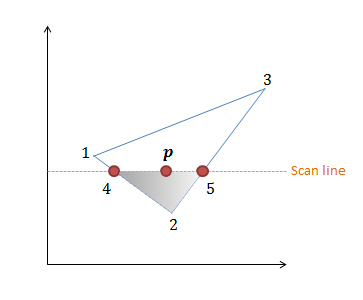
\includegraphics{pics/gouraudInterpolation.png}}
	\caption{Linear interpolation along a scanline}
	\label{fig:gInt}
\end{figure}

\begin{figure}[thbp]
	\centering
	\scalebox{0.7}
	{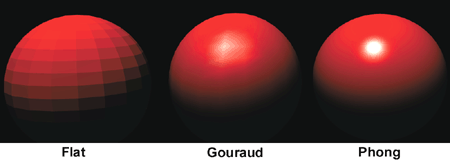
\includegraphics{pics/flatVsGouraudVsPhong.png}}
	\caption{flat vs Gouraud vs Phong shading}
	\label{fig:fVsP}
\end{figure}
